%\documentclass[red, hyperref={pdfpagelabels=false}]{beamer}
\documentclass[red]{beamer}
\hypersetup{pdfpagemode=FullScreen}

\mode<presentation>
\usepackage{beamerthemesplit}
\usepackage[T1]{fontenc}
\usepackage{textcomp}
\usepackage{lmodern}
\usepackage{siunitx}
%\usepackage{listings,bera}
%\usepackage{color}

%\usetheme{boxes}
%\usetheme{Darmstadt}
\usetheme{Dresden}
%\usetheme{Frankfurt}
%\usetheme{Ilmenau}
%\usetheme{Madrid}
%\usetheme{Warsaw}

\title{Examining the Errors in Dual-Polarization Attenuation Correction}
\author{Ryan May}
%\institute{ARRC}
\date{27 February 2014}
\titlegraphic{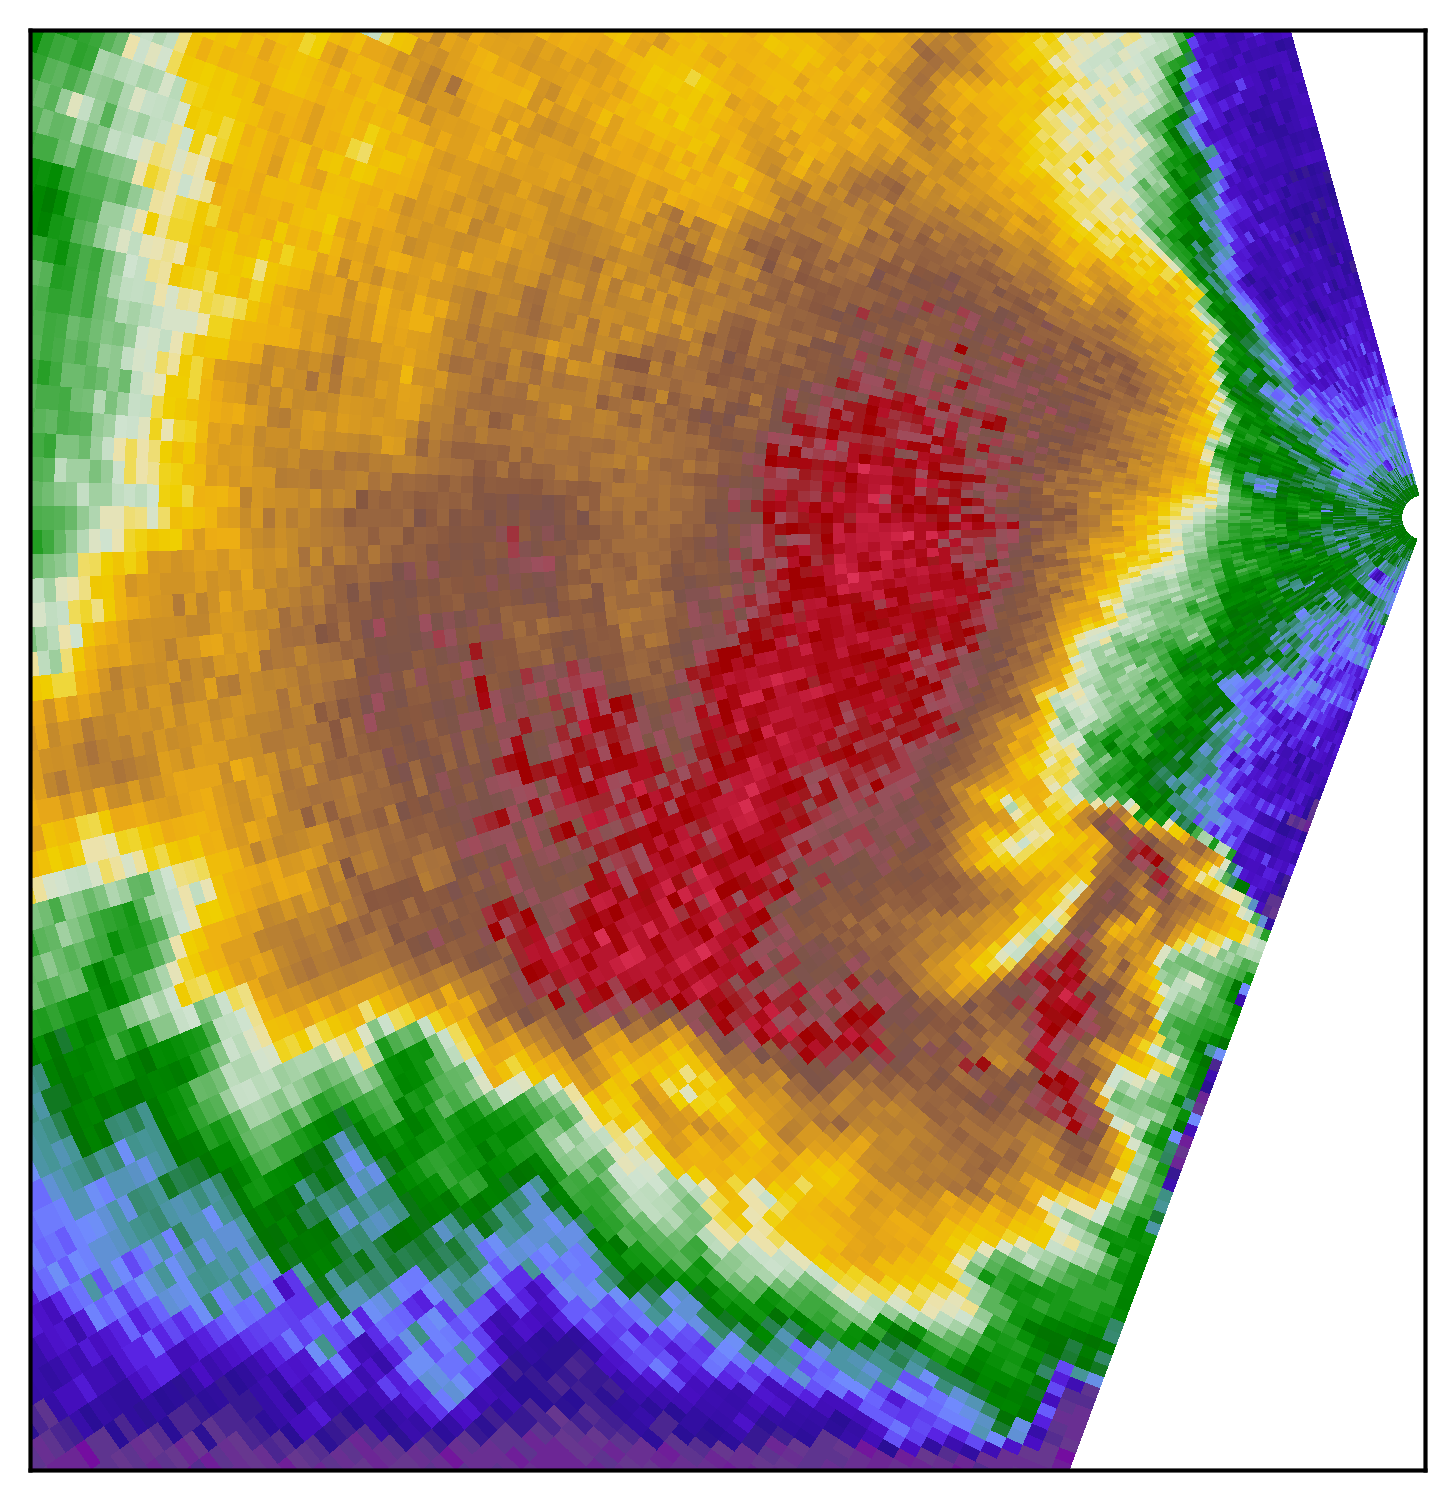
\includegraphics[scale=0.17]{figures/title_ppi.png}}

\begin{document}

\begin{frame}
	\titlepage
\end{frame}

\begin{frame}{Outline}
    \tableofcontents
\end{frame}

\section{Motivation}
\stepcounter{subsection}
\begin{frame}
	\frametitle{Attenuating Systems}
	\begin{itemize}
		\item Proliferation of systems at attenuating wavelengths (C and X bands)
		\item Can be cheaper
		\item Better angular resolution
		\item Better sensitivity
	\end{itemize}
\end{frame}

\begin{frame}
	\frametitle{Applications}
	\begin{itemize}
		\item Any quantitative use of the data necessitates correction for attenuation
		\item QPE
		\item Hydrometeor Classification
		\item 3dB error -> 64\% change in rain rate
	\end{itemize}
\end{frame}

\begin{frame}
	\frametitle{Attenuation Correction}
	\begin{itemize}
		\item Many different algorithms in the literature
		\item Ones examined here
		\begin{itemize}
			\item Linear $\Phi_{DP}$
			\item ZPHI
			\item Self-Consistent
			\item Fully Self-Consistent
		\end{itemize}
		\item All of these rely upon empirically determined coefficients
		\item Which necessitates making certain assumptions (temperature,
		DSD, shape, etc.)
	\end{itemize}
\end{frame}

\begin{frame}
	\frametitle{Testing Corrections}
	\begin{itemize}	
		\item Testing of these techniques usually rely upon comparison with
		unattenuated (S-band) data
		\item Another method involves examining reduction in QPE bias upon correction
		\item Instead here we use simulated data to provide data with and without
		attenuation
		\item Simulator allows changing assumptions to see impacts on correction
	\end{itemize}
\end{frame}

\section{Simulation}
\stepcounter{subsection}
\begin{frame}
  \frametitle{Simulator}
  \begin{itemize}
  	\item Model provides needed environmental information
  	\only<2>{ \begin{itemize}
  		\item Hydrometeor content
  		\item Wind components
  		\item Thermodynamic information
  		\end{itemize} }
  	\item Propagate discretized radar pulse through simulation grid
  	\item During propagation, accumulate phase shift and attenuation
  	\item Calculate scattering parameters from hydrometeor information and temperature
  	\item Use scattering together with radar equation to synthesize radar signal
  	\item Includes antenna pattern (with optional sidelobes), range weighting, and noise
  	\item Also calculate some volume integrated quantities (e.g. attenuation)
  \end{itemize}
\end{frame}

\begin{frame}
	\frametitle{Signal Synthesis}
	\begin{itemize}
		\item Each pulse element gets assigned values from the model grid using nearest
		neighbor sampling
		\item Start each element with uniformly distributed random phases
		\item Each element functions as "scattering center" that generates
		a phase shift (Muschinski 1999)
		\item Power at each element is exponentially distributed with expected value
		given from scattering 
		\item Correlation between polarizations uses scattering calculation
		to adjust randomness between polarizations (Galati 1995)
		\item Each polarization is attenuated and phase-shifted separately
		\item Altogether, this gives complex, random values for each pulse element for 
		each polarization
		\item These are summed and added to white noise for an IQ sample for the pulse
	\end{itemize}
\end{frame}

\begin{frame}
	\frametitle{Scattering}
	\begin{itemize}
		\item Configurable scattering models
		\begin{itemize}
			\item T-Matrix
			\item Rayleigh-Gans
			\item Mie
			\item Rayleigh
			\end{itemize}
		\item Configurable drop shape model
		\begin{itemize}
			\item Brandes et al. (2004) polynomial model
			\item Pruppacher and Beard (1970) linear model
			\end{itemize}
		\item Wavelength- and temperature-dependent complex dielectric constant
		\item Width of canting angle distribution can also be controlled
	\end{itemize}
\end{frame}

\begin{frame}
	\frametitle{Microphysics}
	\begin{itemize}
		\item Native model microphysics scheme is two-moment (Ziegler 1985)
		\item Model distribution is a gamma distribution for volume of drops
		\item However this distribution is not well-suited to radar
		\item Use modified gamma distribution on diameter ($\mu=1.8102$)
		\item This uses the model's number concentration and liquid water content
		\item Also conserves model's $D^6$ (or $V^2$)
	\end{itemize}
\end{frame}

\begin{frame}
	\frametitle{Microphysics (cont.)}
	\begin{center}
		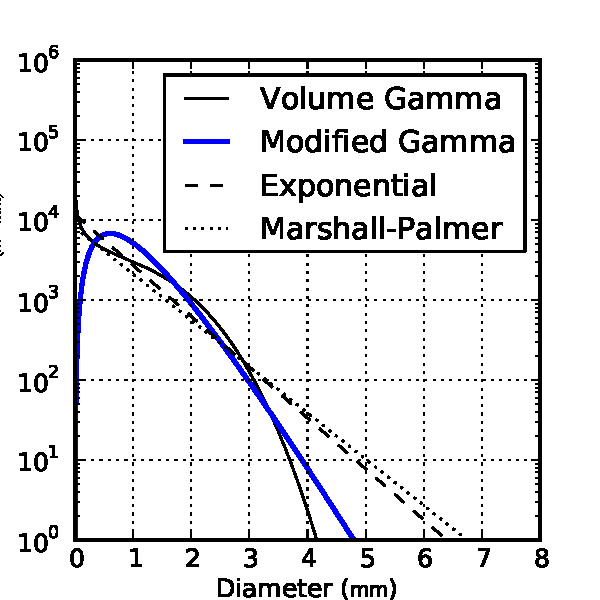
\includegraphics[scale=0.6]{figures/distribution-comparison.pdf}
	\end{center}
\end{frame}

\section{Example Output}
\stepcounter{subsection}
\begin{frame}
	\frametitle{Model Field}
	\begin{center}
		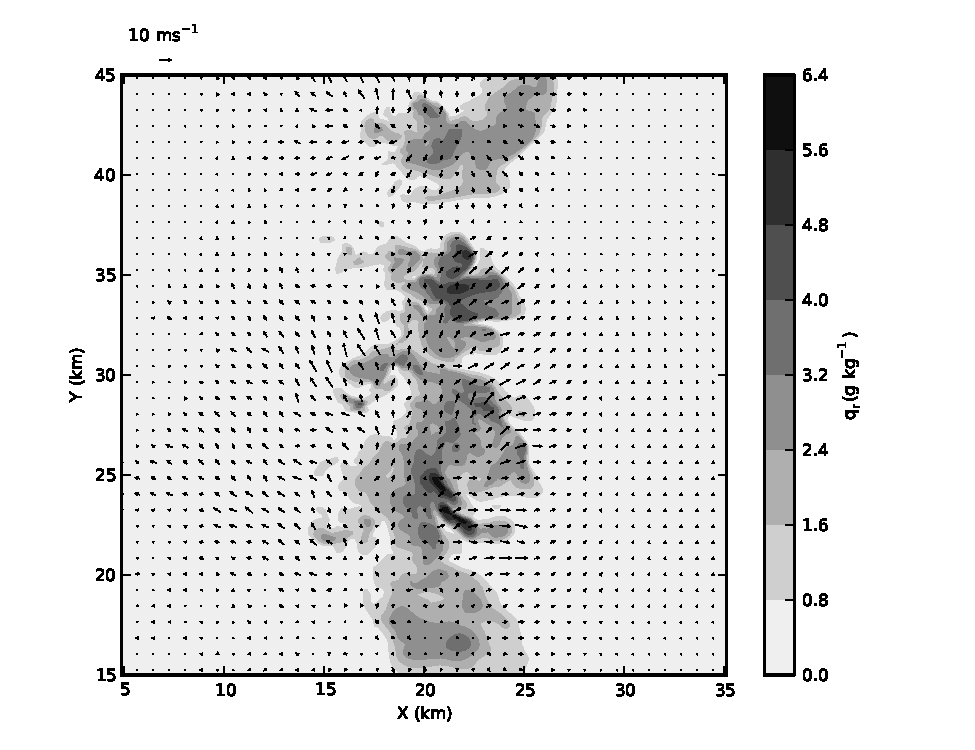
\includegraphics[scale=0.5]{figures/commas_wz_3600_qr_wind_vectors.pdf}	
	\end{center}
\end{frame}

\begin{frame}
	\frametitle{Example Configuration}
	\begin{center}
	    \begin{tabular}{ | l | l | }
	        \hline
	        Antenna gain & \SI{45.5}{dB} \\
	        Peak power & \SI{250}{\kilo\watt} \\
	        First range gate & \SI{500}{\meter} \\
	        Noise power & \SI{-113}{dBm} \\
	        Elevation & \SI{0.5}{\degree} \\
	        PRT & \SI{0.667}{\milli\second} \\
	        Rotation Rate & \SI{20}{\degree\per\second} \\
	        Pulses per radial & \num{75} \\
	        Gate length & \SI{125}{\meter} \\
	        Antenna Limits & Main-lobe only \\
			Wavelength &  \SI{5.5}{\centi\meter} \\
			Beamwidth & \SI{1.0}{\degree} \\
			Radial Spacing & \SI{1.0}{\degree} \\
			\hline
	    \end{tabular}
	\end{center}
\end{frame}

\begin{frame}
	\frametitle{Example Images}
\end{frame}

\begin{frame}
	\frametitle{Example Images (cont.)}
\end{frame}

\begin{frame}
	\frametitle{Example Images (cont.)}
\end{frame}

\begin{frame}
	\frametitle{Example Images (cont.)}
\end{frame}

\section{Correction Algorithms}
\stepcounter{subsection}
\begin{frame}
	\frametitle{Linear $\Phi_{DP}$}
	\begin{itemize}
		\item Described by Bringi et al. (1990)
		\item Formulate linear relationship between $K_{DP}$ and $A_H$
		\begin{align*}
			A_H &= \beta_H K_{DP} \\
			A_D &= \beta_D K_{DP}
		\end{align*}
		\item Leads to direct conversion between $\Phi_{DP}$  and  both
				$\alpha_H$ and $\alpha_D$
	\end{itemize}
\end{frame}

\begin{frame}
	\frametitle{ZPHI}
	\begin{itemize}
		\item Described by Testud et al. (2000)
		\item Based around Hitschfeld (1954) reflectivity-based method
		\item Uses linear $\Phi_{DP}$ to provide constraint
			\begin{align*}
			I(r, r_0) &= \num{0.46}b\int_r^{r_0}Z_a^b(s)\,ds \\
			\alpha(r_0) &= \frac{Z_a^b(r_0)}{I(r_1,r_0)} \lbrace 10^{\num{0.1}b\gamma\Delta\Phi} - 1\rbrace \\
			\alpha(r) &= \frac{Z_a^b(r)}{I(r_1,r_0) + \lbrace 10^{\num{0.1}b\gamma\Delta\Phi} - 1\rbrace I(r, r_0)}
			  \times \lbrace 10^{\num{0.1}b\gamma\Delta\Phi} - 1\rbrace
			\end{align*}
	\end{itemize}
\end{frame}

\begin{frame}
	\frametitle{Self-Consistent}
	\begin{itemize}
		\item Described by Bringi et al. (2001)
		\item Adds a "self-consistent" restriction to ZPHI
		\item Attempts to automatically find the optimal value of $\gamma$
			 \begin{align*}
			\phi_{DP}^c(r;\gamma) &= 2 \int_{r_0}^r \frac{A_h(s;\gamma)}{\gamma}\,ds \\
			\gamma_{min} &\leq \gamma \leq \gamma_{max} \\
			Error &= \sum_{j=1}^N \left| \Phi_{DP}^{filt}(r_j) - \Phi_{DP}^c(r_j;\gamma) \right|
			\end{align*}
	\end{itemize}
\end{frame}

\begin{frame}
		\frametitle{Fully Self-Consistent}
		\begin{itemize}
			\item Described by Gorgucci et al. (2007)
			\item Uses iterative procedure to estimate both attenuation and differential attenuation simultaneously
			\item Estimate a $\Phi_{DP}$ profile from attenuation and compare to
			actual data
			\begin{align*}
			\alpha_d &= \epsilon \alpha_h \\
			K_{dp} &= \left[ \frac{\alpha_h}{a_h Z_h^{b_h} Z_{dr}^{c_h}} \right]^{1/d_h} \\
			K_{dp} &= \left[ \frac{\alpha_d}{a_d Z_h^{b_d} Z_{dr}^{c_d}} \right]^{1/d_d} \\
			\min(\Delta h) &= \min \left\lbrace \int_{r_0}^r \gamma_h \Phi^{h}_{dp}(s) - [\Phi_{dp}(s) - \Phi_{dp}(r_0)]\,ds \right\rbrace \\
			\min(\Delta d) &= \min \left\lbrace \int_{r_0}^r \gamma_d \Phi^{d}_{dp}(s) - [\Phi_{dp}(s) - \Phi_{dp}(r_0)]\,ds \right\rbrace \\
			\widetilde{\alpha}_h &= \gamma_h ^{d_h} \alpha_h \\
			\widetilde{\alpha}_d &= \gamma_h ^{d_d} \alpha_d
			\end{align*}
		\end{itemize}
\end{frame}

\begin{frame}
	\frametitle{Coefficient Regression}
	\begin{itemize}
		\item Need to determine own set of coefficients for algorithms
		\item Original algorithms all use different assumptions
		\item All relations some kind of power law
		\item Make best-case coefficients using actual data from model and
		the assumptions used in simulation
	\end{itemize}
\end{frame}

\begin{frame}
	\frametitle{Coefficient Regression (cont.)}
	\begin{center}
		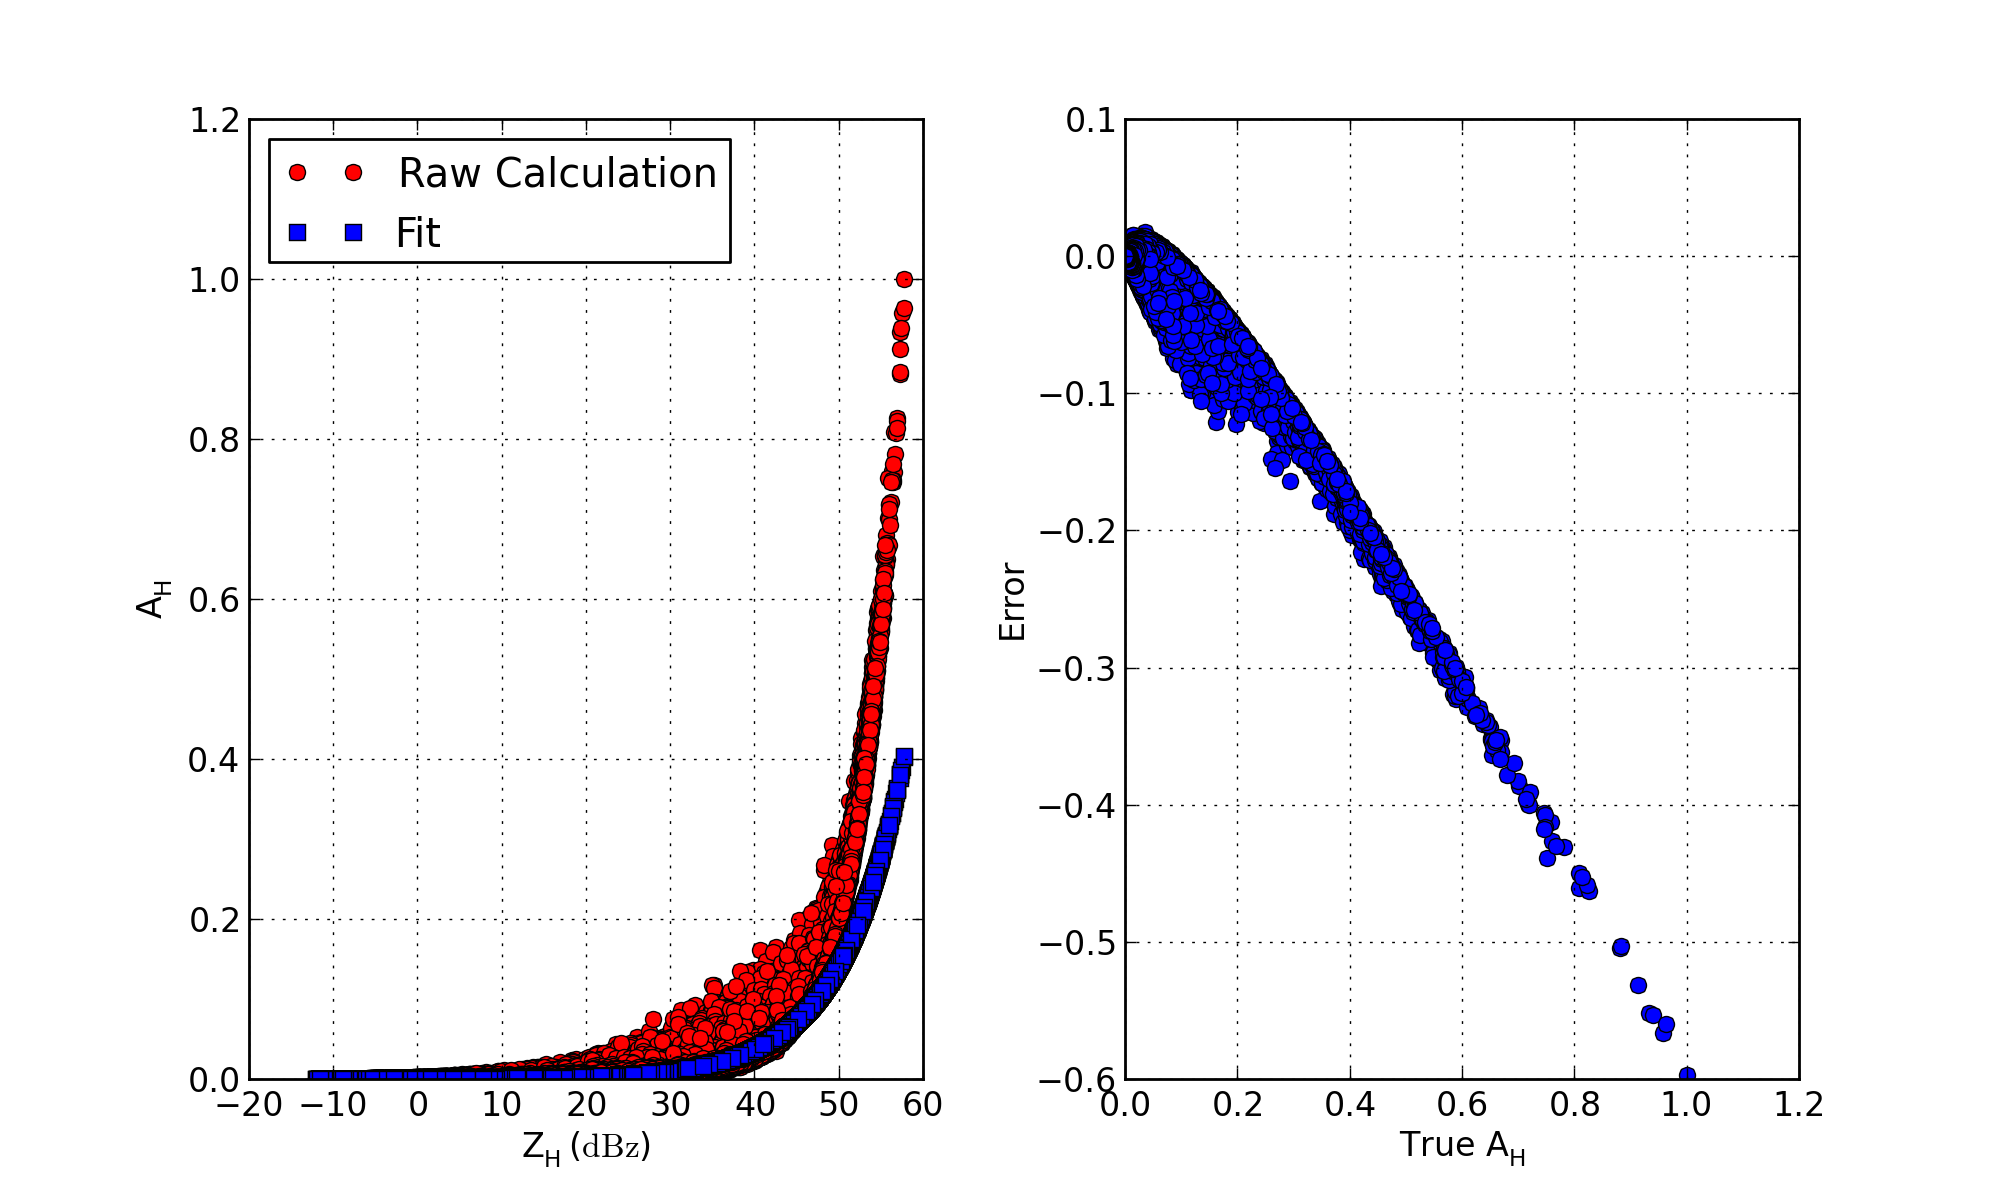
\includegraphics[scale=0.35]{figures/basic_power_law.png}
	\end{center}
	\begin{itemize}
		\item Clearly bias in the fit curve
	\end{itemize}
\end{frame}

\begin{frame}
	\frametitle{Coefficient Regression (cont.)}
	\begin{center}
		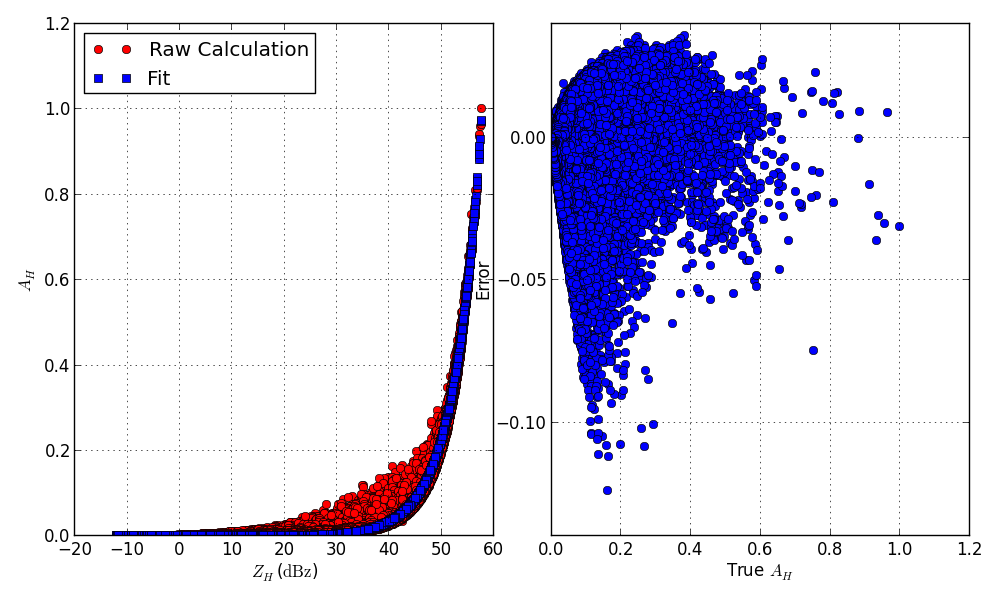
\includegraphics[scale=0.35]{figures/weighted_power_law.png}
	\end{center}
	\begin{itemize}
		\item Much better when using $A_H^2$ as the weights in regression
	\end{itemize}
\end{frame}

\section{Errors}
\stepcounter{subsection}
\subsection{Model Errors}
\begin{frame}
	\frametitle{Experimental Configuration}
	\begin{center}
	    \begin{tabular}{ | l | l | }
	        \hline
	        Antenna gain & \SI{45.5}{dB} \\
	        Peak power & \SI{250}{\kilo\watt} \\
	        First range gate & \SI{500}{\meter} \\
	        Noise power & \SI{-113}{dBm} \\
	        Elevation & \SI{0.5}{\degree} \\
	        PRT & \SI{0.667}{\milli\second} \\
	        Rotation Rate & \SI{20}{\degree\per\second} \\
	        Pulses per radial & \num{75} \\
	        Gate length & \SI{100}{\meter} \\
	        Antenna Limits & Main-lobe only \\
			Beamwidth & \SI{0.25}{\degree} \\
			Radial Spacing & \SI{0.25}{\degree} \\
			Scattering Model & T-Matrix \\
			\hline
	    \end{tabular}
	\end{center}
\end{frame}

\begin{frame}
	\frametitle{Good Assumptions}
	\begin{center}
	    \begin{tabular}{ | l | l | }
	        \hline
	        Temperature & \SI{283}{\kelvin} \\
	        Drop Shape Model & Brandes \\
	        Wavelength & \SI{5.5}{\centi\meter} / \SI{3.2}{\centi\meter} \\
			\hline
	    \end{tabular}
	\end{center}	
\end{frame}

\begin{frame}
	\frametitle{Wavelength}
	\begin{center}
	    \begin{tabular}{ | l | l | }
	        \hline
	        Temperature & \SI{283}{\kelvin} \\
	        Drop Shape Model & Brandes \\
	        Wavelength & \SI{5.0}{\centi\meter} / \SI{3.0}{\centi\meter} \\
			\hline
	    \end{tabular}
	\end{center}	
\end{frame}

\begin{frame}
	\frametitle{Temperature}
	\begin{center}
	    \begin{tabular}{ | l | l | }
	        \hline
	        Temperature & Model Field (\SI{283}{\kelvin}) \\
	        Drop Shape Model & Brandes \\
	        Wavelength & \SI{5.5}{\centi\meter} / \SI{3.2}{\centi\meter} \\
			\hline
	    \end{tabular}
	\end{center}	
\end{frame}

\begin{frame}
	\frametitle{Drop Shape Model}
	\begin{center}
	    \begin{tabular}{ | l | l | }
	        \hline
	        Temperature & \SI{283}{\kelvin} \\
	        Drop Shape Model & Pruppacher \\
	        Wavelength & \SI{5.5}{\centi\meter} / \SI{3.2}{\centi\meter} \\
			\hline
	    \end{tabular}
	\end{center}	
\end{frame}

%\begin{frame}
%	\frametitle{Canting}
%\end{frame}

\begin{frame}
	\frametitle{Worst Case}
	\begin{center}
	    \begin{tabular}{ | l | l | }
	        \hline
	        Temperature & Model Field (\SI{283}{\kelvin}) \\
	        Drop Shape Model & Pruppacher \\
	        Wavelength & \SI{5.0}{\centi\meter} / \SI{3.0}{\centi\meter} \\
			\hline
	    \end{tabular}
	\end{center}	
\end{frame}

%\subsection{Spatial Sampling Errors}
%\begin{frame}
%	\frametitle{Experimental Configuration}
%\end{frame}
%
%\begin{frame}
%	\frametitle{Base Configuration}
%\end{frame}
%
%\begin{frame}
%	\frametitle{Sidelobes}
%\end{frame}
%
%\begin{frame}
%	\frametitle{Increased Beamwidth}
%\end{frame}
%
%\begin{frame}
%	\frametitle{Bigger Radials}
%\end{frame}
%
%\begin{frame}
%	\frametitle{Increased Gatewidth}
%\end{frame}
%
%\begin{frame}
%	\frametitle{Spatial and Modelling Errors}
%\end{frame}

\begin{frame}
	\frametitle{Conclusions}
\end{frame}

\begin{frame}
	\frametitle{Thanks}
	
	\begin{center}
		\large{Questions?}
	\end{center}
\end{frame}

\end{document}
